%% Unfortunately for the contents to contain
%% the "Parts" lines successfully, hyperref
%% needs to be disabled.
\documentclass[nohyper,nobib,openany]{tufte-book}
\usepackage{nameref}
% \hypersetup{colorlinks}% uncomment this line if you prefer colored hyperlinks (e.g., for onscreen viewing)
\setcounter{secnumdepth}{2}

% \usepackage{hyphenat}
\usepackage{url}
\usepackage[backend=biber, natbib=true, style=numeric]{biblatex}
\addbibresource{refs.bib}
\usepackage{xargs}
\renewcommandx{\cite}[3][1={0pt},2={}]{\sidenote[][#1]{\fullcite[#2]{#3}}}

%%
% Book metadata
\title{Machine Learning in Feedback Systems}
\date{Fall 2023}
\author[CS 6784 taught by Sarah Dean]{CS 6784 taught by Sarah Dean}
\publisher{Cornell University Computer Science Department}


%%
% If they're installed, use Bergamo and Chantilly from www.fontsite.com.
% They're clones of Bembo and Gill Sans, respectively.
%\IfFileExists{bergamo.sty}{\usepackage[osf]{bergamo}}{}% Bembo
%\IfFileExists{chantill.sty}{\usepackage{chantill}}{}% Gill Sans

%\usepackage{microtype}

%%
% Just some sample text
\usepackage{lipsum}

%%
% For nicely typeset tabular material
\usepackage{booktabs}

%%
% For graphics / images
\usepackage{graphicx}
\setkeys{Gin}{width=\linewidth,totalheight=\textheight,keepaspectratio}
\graphicspath{{graphics/}}

% The fancyvrb package lets us customize the formatting of verbatim
% environments.  We use a slightly smaller font.
\usepackage{fancyvrb}
\fvset{fontsize=\normalsize}

%%
% Prints argument within hanging parentheses (i.e., parentheses that take
% up no horizontal space).  Useful in tabular environments.
\newcommand{\hangp}[1]{\makebox[0pt][r]{(}#1\makebox[0pt][l]{)}}

%%
% Prints an asterisk that takes up no horizontal space.
% Useful in tabular environments.
\newcommand{\hangstar}{\makebox[0pt][l]{*}}

%%
% Prints a trailing space in a smart way.
\usepackage{xspace}

% Prints the month name (e.g., January) and the year (e.g., 2008)
\newcommand{\monthyear}{%
  \ifcase\month\or January\or February\or March\or April\or May\or June\or
  July\or August\or September\or October\or November\or
  December\fi\space\number\year
}


% Prints an epigraph and speaker in sans serif, all-caps type.
\newcommand{\openepigraph}[2]{%
  %\sffamily\fontsize{14}{16}\selectfont
  \begin{fullwidth}
  \sffamily\large
  \begin{doublespace}
  \noindent\allcaps{#1}\\% epigraph
  \noindent\allcaps{#2}% author
  \end{doublespace}
  \end{fullwidth}
}

% Inserts a blank page
\newcommand{\blankpage}{\newpage\hbox{}\thispagestyle{empty}\newpage}

\usepackage{units}

% Typesets the font size, leading, and measure in the form of 10/12x26 pc.
\newcommand{\measure}[3]{#1/#2$\times$\unit[#3]{pc}}

% Macros for typesetting the documentation
\newcommand{\hlred}[1]{\textcolor{Maroon}{#1}}% prints in red
\newcommand{\hangleft}[1]{\makebox[0pt][r]{#1}}
\newcommand{\hairsp}{\hspace{1pt}}% hair space
\newcommand{\hquad}{\hskip0.5em\relax}% half quad space
\newcommand{\TODO}{\textcolor{red}{\bf TODO!}\xspace}
\newcommand{\ie}{\textit{i.\hairsp{}e.}\xspace}
\newcommand{\eg}{\textit{e.\hairsp{}g.}\xspace}
\newcommand{\na}{\quad--}% used in tables for N/A cells
\providecommand{\XeLaTeX}{X\lower.5ex\hbox{\kern-0.15em\reflectbox{E}}\kern-0.1em\LaTeX}
\newcommand{\tXeLaTeX}{\XeLaTeX\index{XeLaTeX@\protect\XeLaTeX}}
% \index{\texttt{\textbackslash xyz}@\hangleft{\texttt{\textbackslash}}\texttt{xyz}}
\newcommand{\tuftebs}{\symbol{'134}}% a backslash in tt type in OT1/T1
\newcommand{\doccmdnoindex}[2][]{\texttt{\tuftebs#2}}% command name -- adds backslash automatically (and doesn't add cmd to the index)
\newcommand{\doccmddef}[2][]{%
  \hlred{\texttt{\tuftebs#2}}\label{cmd:#2}%
  \ifthenelse{\isempty{#1}}%
    {% add the command to the index
      \index{#2 command@\protect\hangleft{\texttt{\tuftebs}}\texttt{#2}}% command name
    }%
    {% add the command and package to the index
      \index{#2 command@\protect\hangleft{\texttt{\tuftebs}}\texttt{#2} (\texttt{#1} package)}% command name
      \index{#1 package@\texttt{#1} package}\index{packages!#1@\texttt{#1}}% package name
    }%
}% command name -- adds backslash automatically
\newcommand{\doccmd}[2][]{%
  \texttt{\tuftebs#2}%
  \ifthenelse{\isempty{#1}}%
    {% add the command to the index
      \index{#2 command@\protect\hangleft{\texttt{\tuftebs}}\texttt{#2}}% command name
    }%
    {% add the command and package to the index
      \index{#2 command@\protect\hangleft{\texttt{\tuftebs}}\texttt{#2} (\texttt{#1} package)}% command name
      \index{#1 package@\texttt{#1} package}\index{packages!#1@\texttt{#1}}% package name
    }%
}% command name -- adds backslash automatically
\newcommand{\docopt}[1]{\ensuremath{\langle}\textrm{\textit{#1}}\ensuremath{\rangle}}% optional command argument
\newcommand{\docarg}[1]{\textrm{\textit{#1}}}% (required) command argument
\newenvironment{docspec}{\begin{quotation}\ttfamily\parskip0pt\parindent0pt\ignorespaces}{\end{quotation}}% command specification environment
\newcommand{\docenv}[1]{\texttt{#1}\index{#1 environment@\texttt{#1} environment}\index{environments!#1@\texttt{#1}}}% environment name
\newcommand{\docenvdef}[1]{\hlred{\texttt{#1}}\label{env:#1}\index{#1 environment@\texttt{#1} environment}\index{environments!#1@\texttt{#1}}}% environment name
\newcommand{\docpkg}[1]{\texttt{#1}\index{#1 package@\texttt{#1} package}\index{packages!#1@\texttt{#1}}}% package name
\newcommand{\doccls}[1]{\texttt{#1}}% document class name
\newcommand{\docclsopt}[1]{\texttt{#1}\index{#1 class option@\texttt{#1} class option}\index{class options!#1@\texttt{#1}}}% document class option name
\newcommand{\docclsoptdef}[1]{\hlred{\texttt{#1}}\label{clsopt:#1}\index{#1 class option@\texttt{#1} class option}\index{class options!#1@\texttt{#1}}}% document class option name defined
\newcommand{\docmsg}[2]{\bigskip\begin{fullwidth}\noindent\ttfamily#1\end{fullwidth}\medskip\par\noindent#2}
\newcommand{\docfilehook}[2]{\texttt{#1}\index{file hooks!#2}\index{#1@\texttt{#1}}}
\newcommand{\doccounter}[1]{\texttt{#1}\index{#1 counter@\texttt{#1} counter}}

% Generates the index
\usepackage{makeidx}
\makeindex

%%%% Kevin Godny's code for title page and contents from https://groups.google.com/forum/#!topic/tufte-latex/ujdzrktC1BQ
\makeatletter
\renewcommand{\maketitlepage}{%
\begingroup%
\setlength{\parindent}{0pt}

{\fontsize{24}{24}\selectfont\textit{\@author}\par}

\vspace{1.75in}{\fontsize{36}{54}\selectfont\@title\par}

\vspace{0.5in}{\fontsize{14}{14}\selectfont\textsf{\smallcaps{\@date}}\par}

\vfill{\fontsize{14}{14}\selectfont\textit{\@publisher}\par}

\thispagestyle{empty}
\endgroup
}
\makeatother

\titlecontents{part}%
    [0pt]% distance from left margin
    {\addvspace{0.25\baselineskip}}% above (global formatting of entry)
    {\allcaps{Part~\thecontentslabel}\allcaps}% before w/ label (label = ``Part I'')
    {\allcaps{Part~\thecontentslabel}\allcaps}% before w/o label
    {}% filler and page (leaders and page num)
    [\vspace*{0.5\baselineskip}]% after

\titlecontents{chapter}%
    [4em]% distance from left margin
    {}% above (global formatting of entry)
    {\contentslabel{2em}\textit}% before w/ label (label = ``Chapter 1'')
    {\hspace{0em}\textit}% before w/o label
    {\qquad\thecontentspage}% filler and page (leaders and page num)
    [\vspace*{0.5\baselineskip}]% after
%%%% End additional code by Kevin Godby

\usepackage{amsfonts,amsthm,amsmath,amssymb, cancel}
\DeclareMathOperator*{\argmax}{arg\,max}
\DeclareMathOperator*{\argmin}{arg\,min}
\newtheorem{thm}{Theorem}[section]
\newtheorem{claim}[thm]{Claim}
\newtheorem{fact}[thm]{Fact}
\newtheorem{theorem}[thm]{Theorem}
\newtheorem{lemma}[thm]{Lemma}
\newtheorem{exercise}{Exercise}
\newtheorem{definition}{Definition}

\usepackage{pgfplots}
\usepackage{csquotes}
\usepackage{rotating}
\usepackage{wrapfig}
\usepackage{cleveref}
\usepackage{xcolor}
\usepackage[normalem]{ulem}

\newcommand{\cd}{\cdot}
\newcommand{\p}[1]{\left( #1 \right)}

\newcommand\norm[1]{\left\lVert#1\right\rVert}

\begin{document}

% Front matter
\frontmatter

% r.1 blank page
% \blankpage

% v.2 epigraphs
% \newpage\thispagestyle{empty}
% \openepigraph{%
% The public is more familiar with bad design than good design.
% It is, in effect, conditioned to prefer bad design, 
% because that is what it lives with. 
% The new becomes threatening, the old reassuring.
% }{Paul Rand%, {\itshape Design, Form, and Chaos}
% }
% \vfill
% \openepigraph{%
% A designer knows that he has achieved perfection 
% not when there is nothing left to add, 
% but when there is nothing left to take away.
% }{Antoine de Saint-Exup\'{e}ry}
% \vfill
% \openepigraph{%
% \ldots the designer of a new system must not only be the implementor and the first 
% large-scale user; the designer should also write the first user manual\ldots 
% If I had not participated fully in all these activities, 
% literally hundreds of improvements would never have been made, 
% because I would never have thought of them or perceived 
% why they were important.
% }{Donald E. Knuth}


% r.3 full title page
\maketitle


% % v.4 copyright page
% \newpage
% \begin{fullwidth}
% ~\vfill
% \thispagestyle{empty}
% \setlength{\parindent}{0pt}
% \setlength{\parskip}{\baselineskip}
% Copyright \copyright\ \the\year\ \thanklessauthor

% \par\smallcaps{Published by \thanklesspublisher}

% \par\smallcaps{tufte-latex.googlecode.com}

% \par Licensed under the Apache License, Version 2.0 (the ``License''); you may not
% use this file except in compliance with the License. You may obtain a copy
% of the License at \url{http://www.apache.org/licenses/LICENSE-2.0}. Unless
% required by applicable law or agreed to in writing, software distributed
% under the License is distributed on an \smallcaps{``AS IS'' BASIS, WITHOUT
% WARRANTIES OR CONDITIONS OF ANY KIND}, either express or implied. See the
% License for the specific language governing permissions and limitations
% under the License.\index{license}

% \par\textit{First printing, \monthyear}
% \end{fullwidth}

% r.5 contents
\tableofcontents

% \listoffigures

% \listoftables

% r.7 dedication
% \cleardoublepage
% ~\vfill
% \begin{doublespace}
% \noindent \fontsize{18}{22}\selectfont\itshape
% \nohyphenation
% Dedicated to those who appreciate \LaTeX{} 
% and the work of \mbox{Edward R.~Tufte} 
% and \mbox{Donald E.~Knuth}.
% \end{doublespace}
% \vfill
% \vfill


% r.9 introduction
% \cleardoublepage
% \graphicspath{ {./0-intro/} }
\chapter*{Introduction and Overview}

\begin{marginfigure}%
  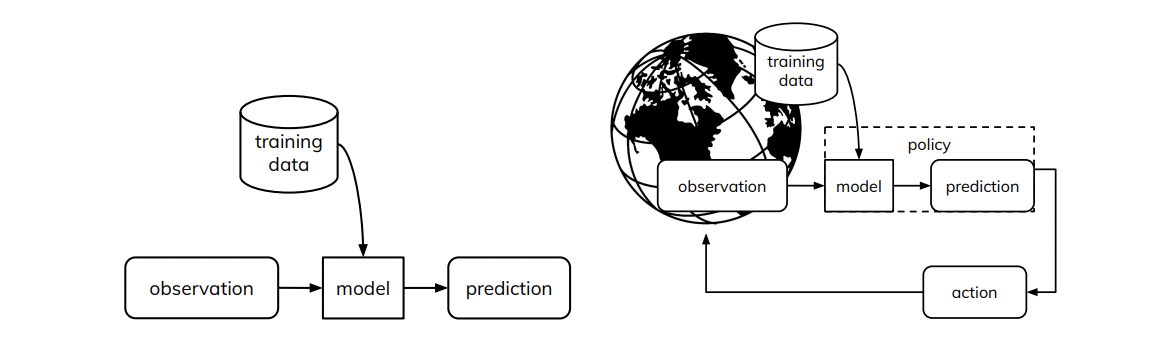
\includegraphics[width=\linewidth]{FeedbackvsTraditional.png}\caption{Though machine learning models are often trained with a static supervised
learning framing in mind (left), when deployed, they become part of a feedback loop
(right).}
  \label{fig:feedback_vs_trad}
\end{marginfigure}

Machine Learning has a lot of predictive power to offer and thus constitutes an amazing potential tool for decision-making. In a traditional setting, an algorithm will output the insights its understood from the data it received allowing a decision-maker to react accordingly. Removing the decision-maker from the loop by building a system that both predicts and decides in a closed loop brings a whole new set of issues to consider. As Machine Learning models are often deployed as part of large applications, the study of these issues is increasingly consequential.

In feedback systems, a policy is used to produce an action that influences the environment.
The policy may contain a model which is learned using training data and/or observations from the environment.
The policy can also be rolled out (inference) using observations from the environment.

\begin{figure}
\centering
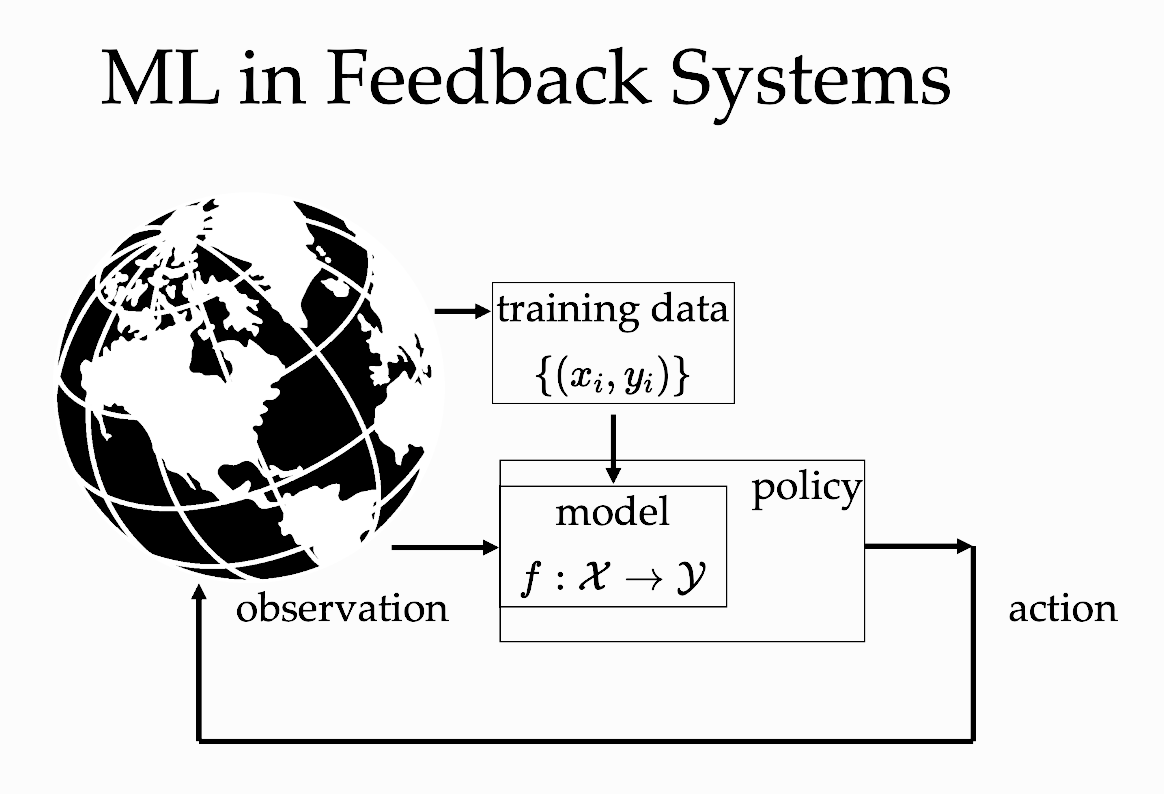
\includegraphics[width=3in]{ml_feedback_sys.png}
\caption{ML in Feedback Systems, from the Lecture 1 slides.}
\end{figure}



\section*{Overview of Machine Learning Frameworks}\label{sec:overview}

% TODO: mention prediction vs. action, online vs. offline, and static vs dynamic

There are four major ML frameworks which we will deal with in this class: Supervised Learning, Online Learning, Contextual Bandits, and Online Control/RL

\subsection*{Supervised Learning}
    
\begin{marginfigure}%
  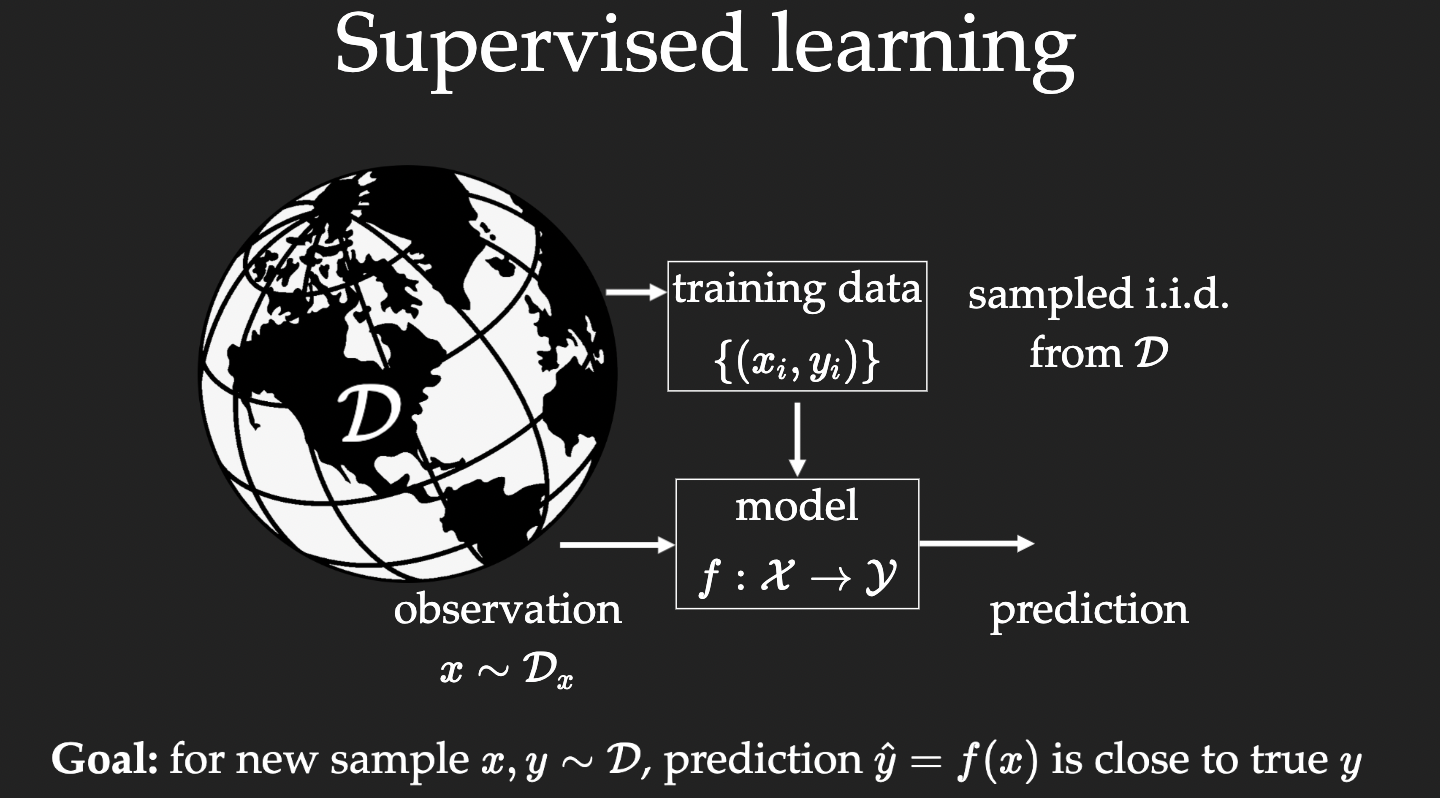
\includegraphics[width=\linewidth]{Supervised_Learning.png}
\caption{The Supervised Learning framework}
  \label{fig:supervised_learning}
\end{marginfigure}
    
In a traditional supervised learning setting, a model is trained by sampling data points i.i.d from the distribution we are hoping to make predictions on. We train a predictive model with this dataset. We are aiming to be able to predict as accurately as possible the unknown label corresponding to the known features with a new sample from this distribution.\\
\subsection*{Online Learning}




\begin{marginfigure}%
  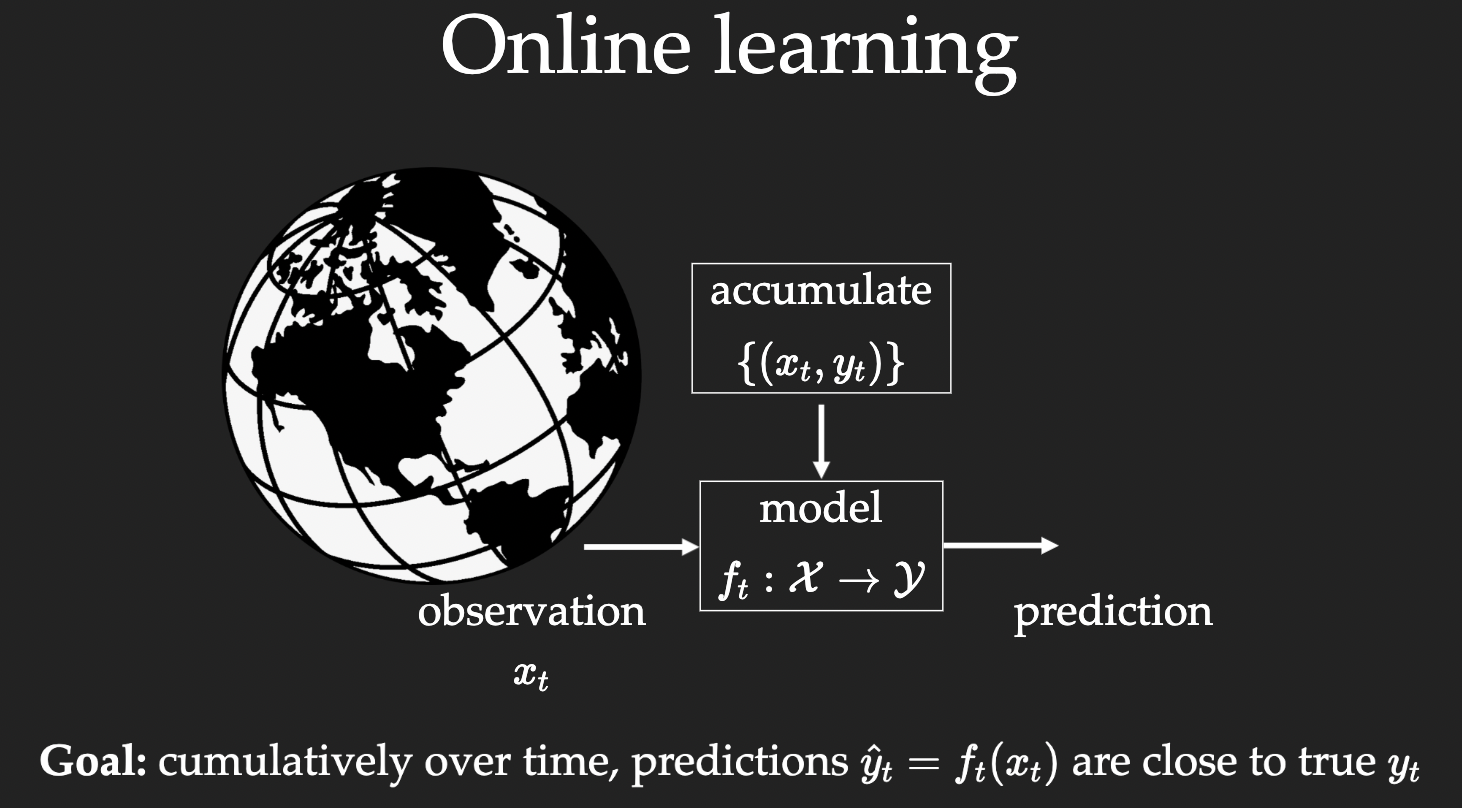
\includegraphics[width=\linewidth]{Online_Learning.png}
\caption{The Online Learning framework}
  \label{fig:online_learning_framework}
\end{marginfigure}

We are now dealing with a framework for which we do not have a fixed set of data points drawn i.i.d from a fixed distribution. Our data points are collected progressively over time and we want to constantly be able to make predictions based on the information that we have gathered so far. 
At each time step t, we get a feature vector $x_t$, we make a prediction of its label $\hat{y}_t$, we then receive the true label $y_t$, which we use to calculate how erroneous our prediction function is and use that information to update our model $f_t$.

\subsection*{Contextual bandits}
    
\begin{marginfigure}%
  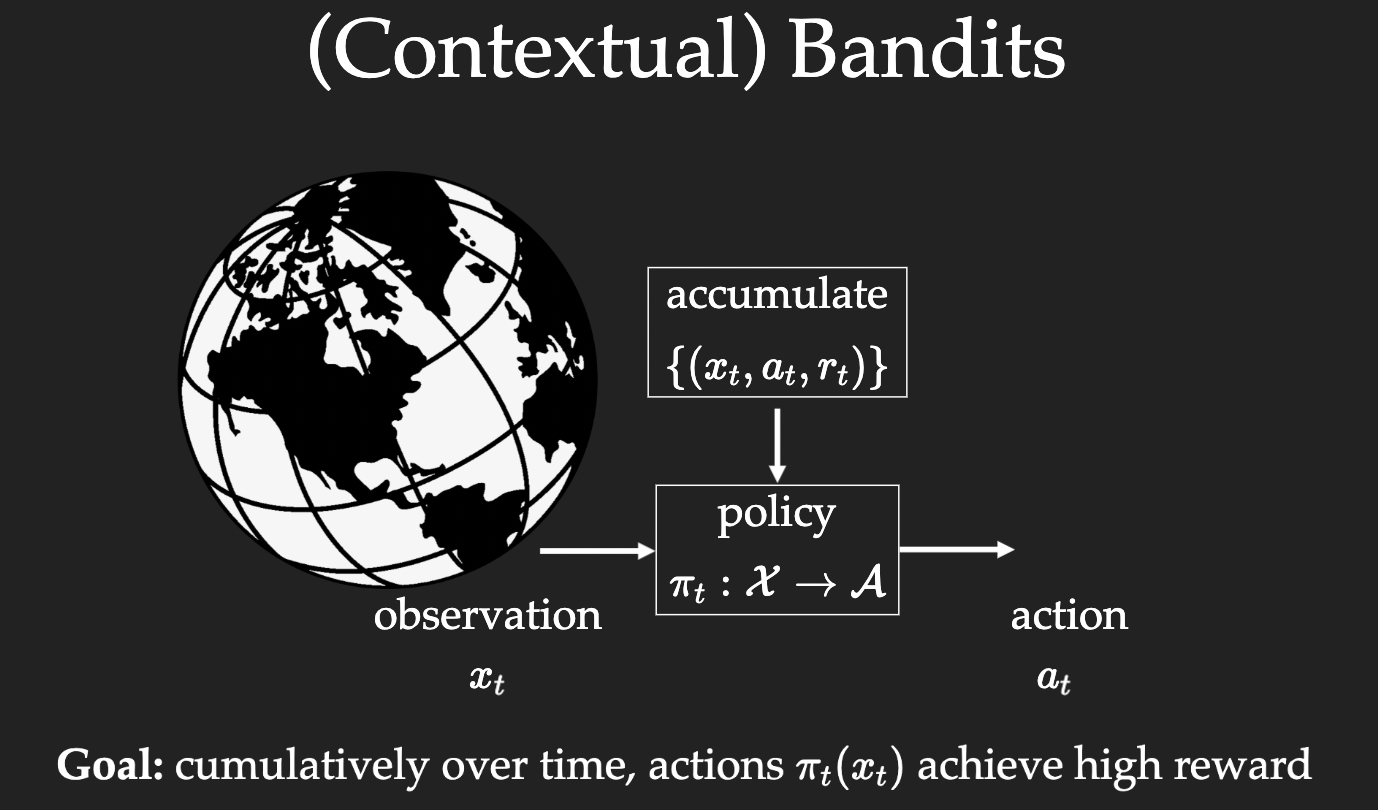
\includegraphics[width=\linewidth]{Contextual_Bandits.png}
\caption{The Contextual Bandits framework}
  \label{fig:contextual_bandits_framework}
\end{marginfigure}
    

In the setting of contextual bandits, similarly to the Online Learning setting we are not dealing with a fixed set of data points coming from a fixed distribution. To this we add another difference: we no longer wish to accurately predict the label of an input vector using a predictive model; instead we wish to learn a policy - a function that will map a context (an input vector) to an action (or an arm). We are no longer trying to minimize a loss function but we want to maximize a cumulative reward. Just like accuracy is the metric in supervised learning, here the metric is the reward - how good or bad this action was for our specific overall objective. Just like the online learning setting these updates to our policy are made progressively as time passes and we accumulate more and more data points. In a given context $x_t$ we take an action $a_t$, observe a reward $r_t$, and update our policy $\pi_t$.

\subsection*{Online control / Reinforcement Learning}

\begin{marginfigure}%
  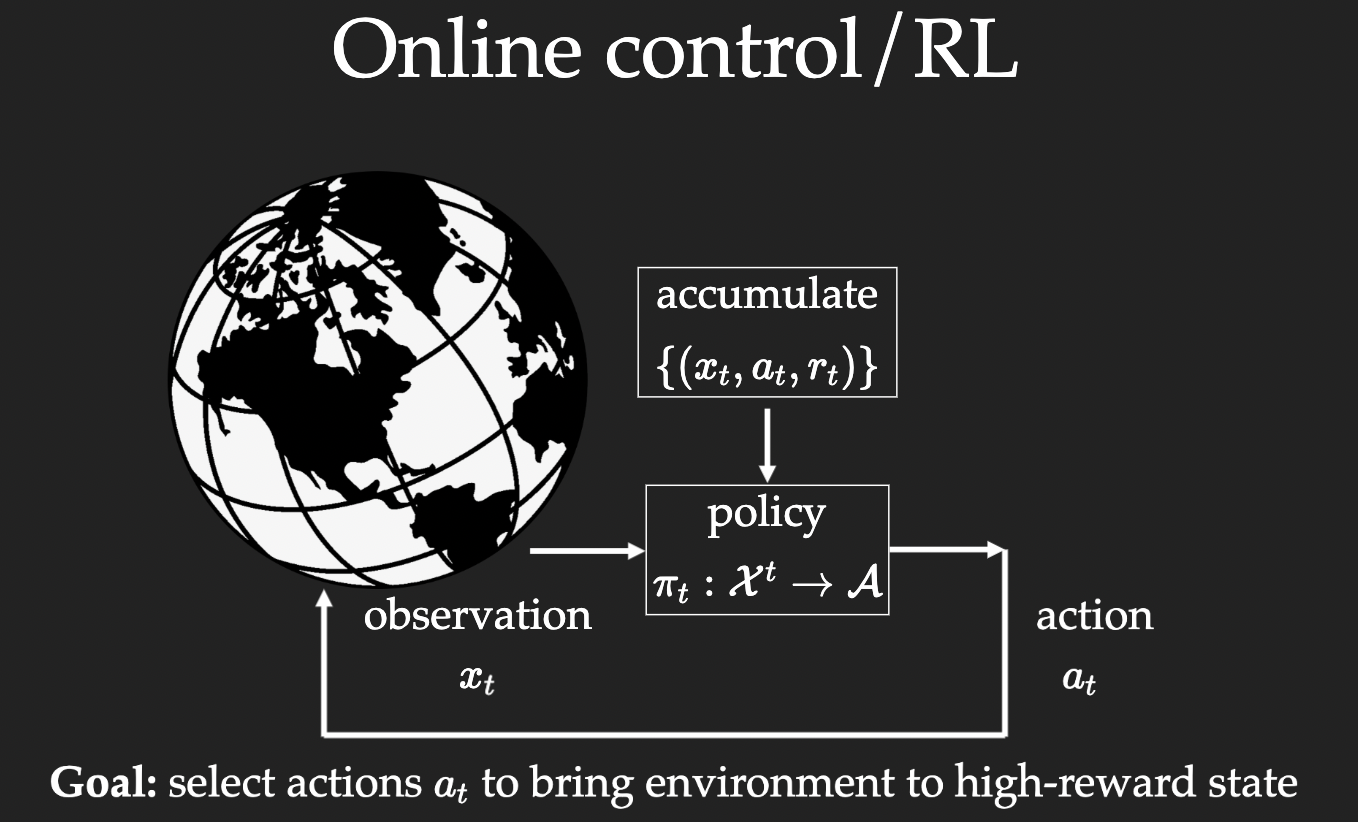
\includegraphics[width=\linewidth]{Online_control.png}
\caption{The Reinforcement Learning framework}
  \label{fig:reinforcement_learning_framework}
\end{marginfigure}

% \begin{figure}[h]
% \centering
% 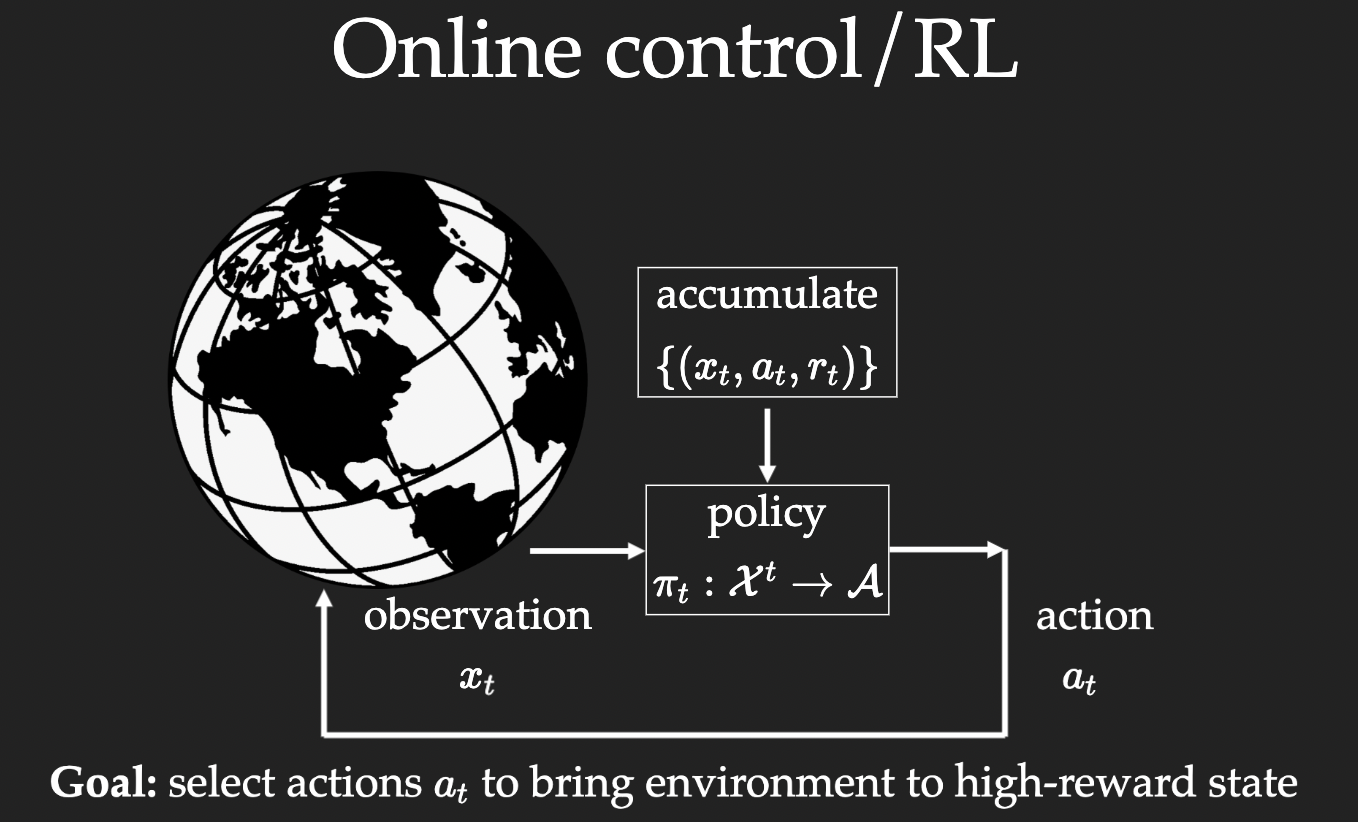
\includegraphics[width=\linewidth]{Online_control.png}
% \caption{The Reinforcement Learning framework}
% \end{figure}\\
Finally, in the setting of Online Control/Reinforcement Learning, we are still in the context of an accumulation of data points that we use to progressively update a policy. However, the big difference with the previous setting is that the environment changes with respect to our actions. We observe a state $x_t$ from a distribution $\chi_t$, pick an action $a_t$ based on our policy $\pi_t$, observe a reward $r_t$ that we use to update our policy. At time $t+1$ however the new state of our environment $x_{t+1}$ is coming from a distribution $\chi_{t+1}$.

\marginnote{Originally scribed by Eliot Shekhtman \& Yann Hicke on August 22nd, 2022}


%%
% Start the main matter (normal chapters)
\mainmatter

\graphicspath{ {./0-intro/} }
\chapter*{Introduction and Overview}

\begin{marginfigure}%
  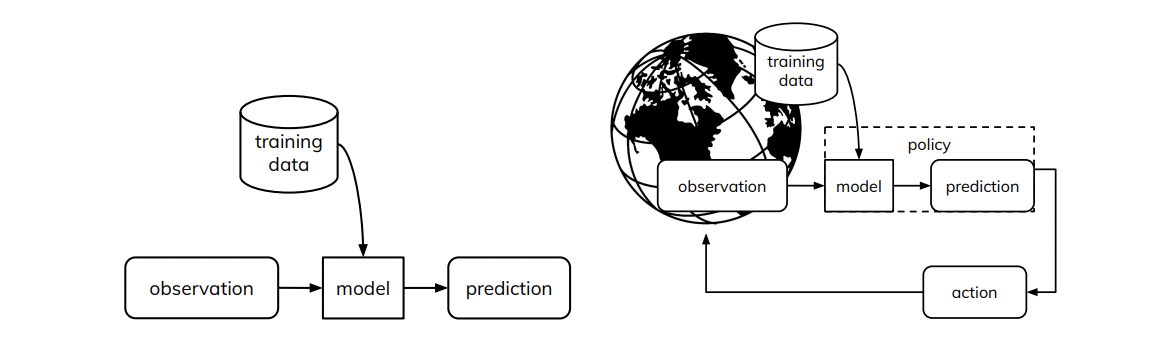
\includegraphics[width=\linewidth]{FeedbackvsTraditional.png}\caption{Though machine learning models are often trained with a static supervised
learning framing in mind (left), when deployed, they become part of a feedback loop
(right).}
  \label{fig:feedback_vs_trad}
\end{marginfigure}

Machine Learning has a lot of predictive power to offer and thus constitutes an amazing potential tool for decision-making. In a traditional setting, an algorithm will output the insights its understood from the data it received allowing a decision-maker to react accordingly. Removing the decision-maker from the loop by building a system that both predicts and decides in a closed loop brings a whole new set of issues to consider. As Machine Learning models are often deployed as part of large applications, the study of these issues is increasingly consequential.

In feedback systems, a policy is used to produce an action that influences the environment.
The policy may contain a model which is learned using training data and/or observations from the environment.
The policy can also be rolled out (inference) using observations from the environment.

\begin{figure}
\centering
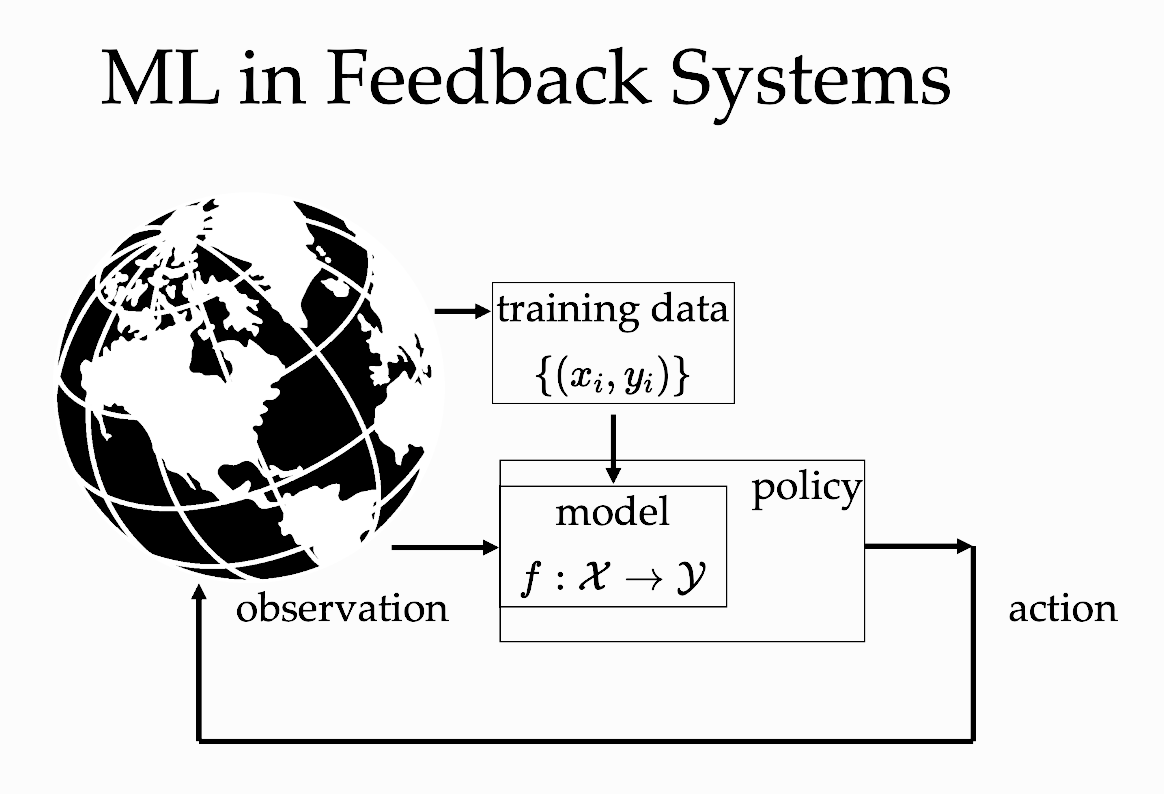
\includegraphics[width=3in]{ml_feedback_sys.png}
\caption{ML in Feedback Systems, from the Lecture 1 slides.}
\end{figure}



\section*{Overview of Machine Learning Frameworks}\label{sec:overview}

% TODO: mention prediction vs. action, online vs. offline, and static vs dynamic

There are four major ML frameworks which we will deal with in this class: Supervised Learning, Online Learning, Contextual Bandits, and Online Control/RL

\subsection*{Supervised Learning}
    
\begin{marginfigure}%
  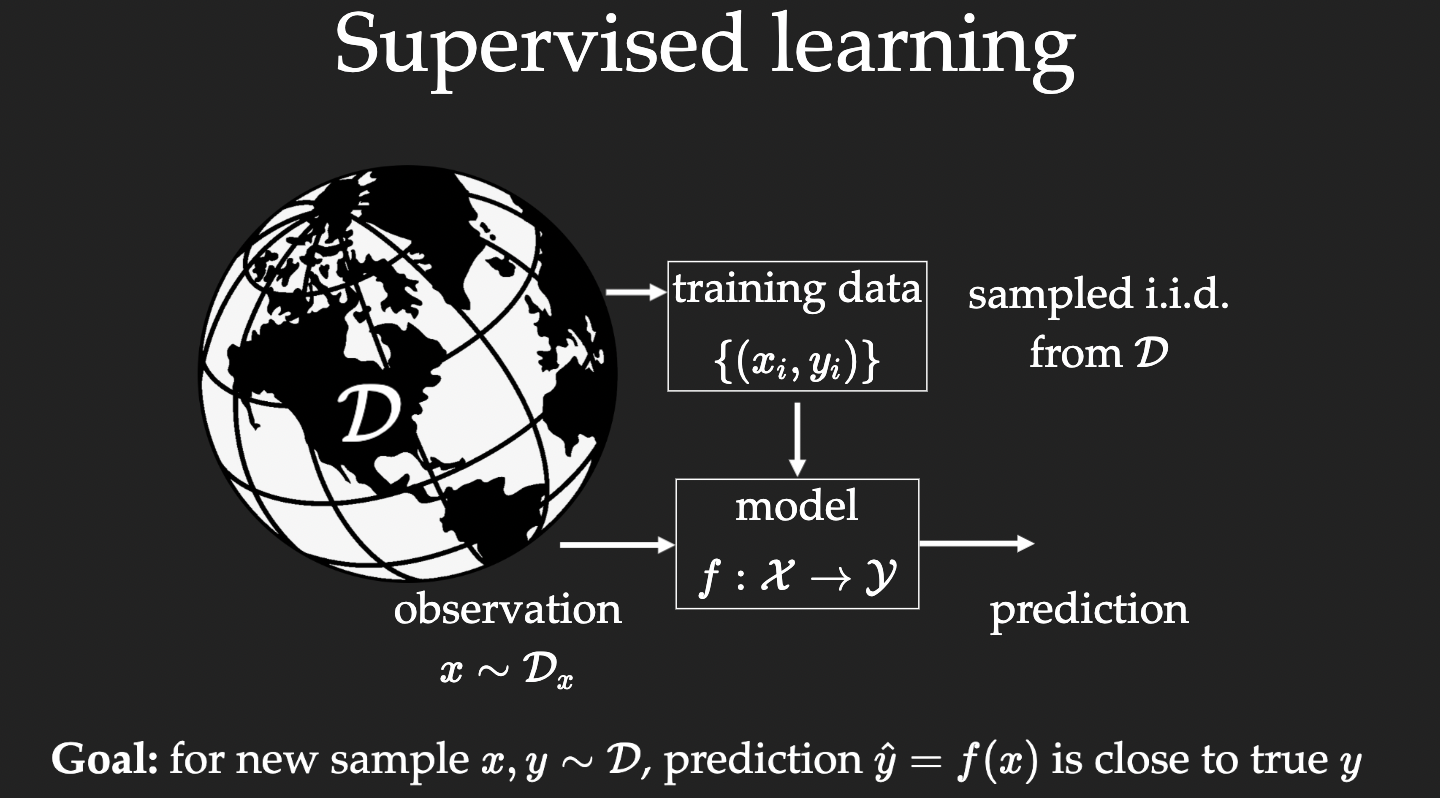
\includegraphics[width=\linewidth]{Supervised_Learning.png}
\caption{The Supervised Learning framework}
  \label{fig:supervised_learning}
\end{marginfigure}
    
In a traditional supervised learning setting, a model is trained by sampling data points i.i.d from the distribution we are hoping to make predictions on. We train a predictive model with this dataset. We are aiming to be able to predict as accurately as possible the unknown label corresponding to the known features with a new sample from this distribution.\\
\subsection*{Online Learning}




\begin{marginfigure}%
  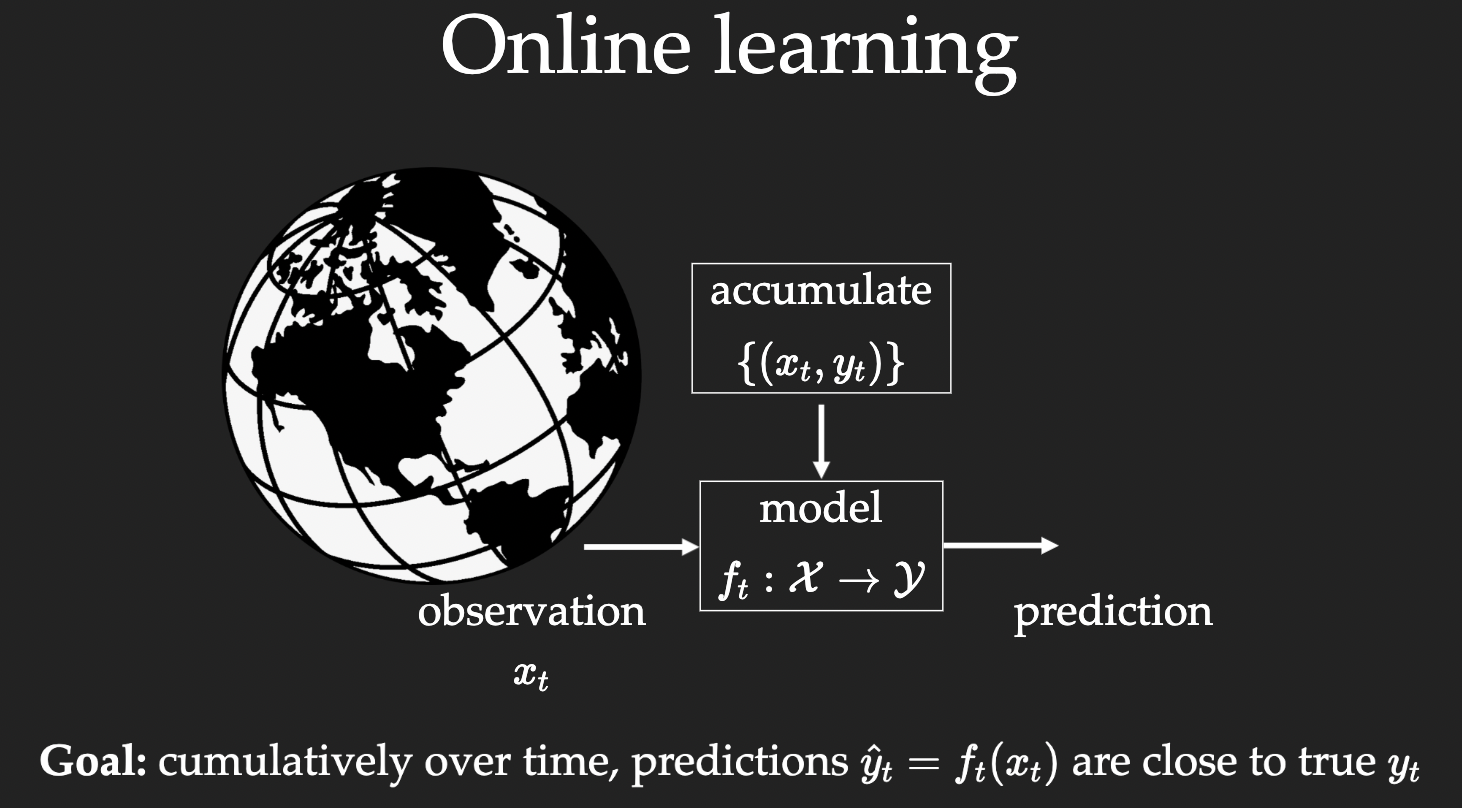
\includegraphics[width=\linewidth]{Online_Learning.png}
\caption{The Online Learning framework}
  \label{fig:online_learning_framework}
\end{marginfigure}

We are now dealing with a framework for which we do not have a fixed set of data points drawn i.i.d from a fixed distribution. Our data points are collected progressively over time and we want to constantly be able to make predictions based on the information that we have gathered so far. 
At each time step t, we get a feature vector $x_t$, we make a prediction of its label $\hat{y}_t$, we then receive the true label $y_t$, which we use to calculate how erroneous our prediction function is and use that information to update our model $f_t$.

\subsection*{Contextual bandits}
    
\begin{marginfigure}%
  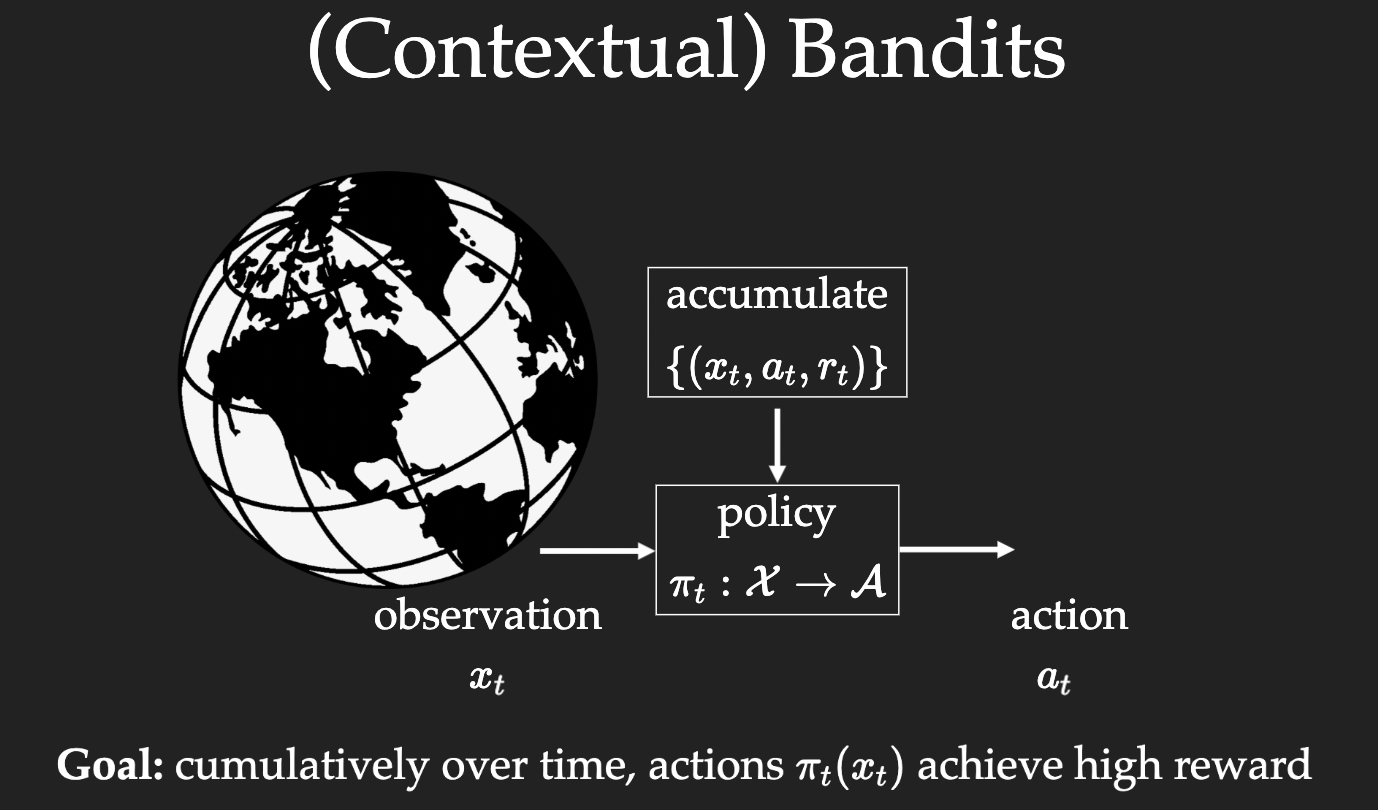
\includegraphics[width=\linewidth]{Contextual_Bandits.png}
\caption{The Contextual Bandits framework}
  \label{fig:contextual_bandits_framework}
\end{marginfigure}
    

In the setting of contextual bandits, similarly to the Online Learning setting we are not dealing with a fixed set of data points coming from a fixed distribution. To this we add another difference: we no longer wish to accurately predict the label of an input vector using a predictive model; instead we wish to learn a policy - a function that will map a context (an input vector) to an action (or an arm). We are no longer trying to minimize a loss function but we want to maximize a cumulative reward. Just like accuracy is the metric in supervised learning, here the metric is the reward - how good or bad this action was for our specific overall objective. Just like the online learning setting these updates to our policy are made progressively as time passes and we accumulate more and more data points. In a given context $x_t$ we take an action $a_t$, observe a reward $r_t$, and update our policy $\pi_t$.

\subsection*{Online control / Reinforcement Learning}

\begin{marginfigure}%
  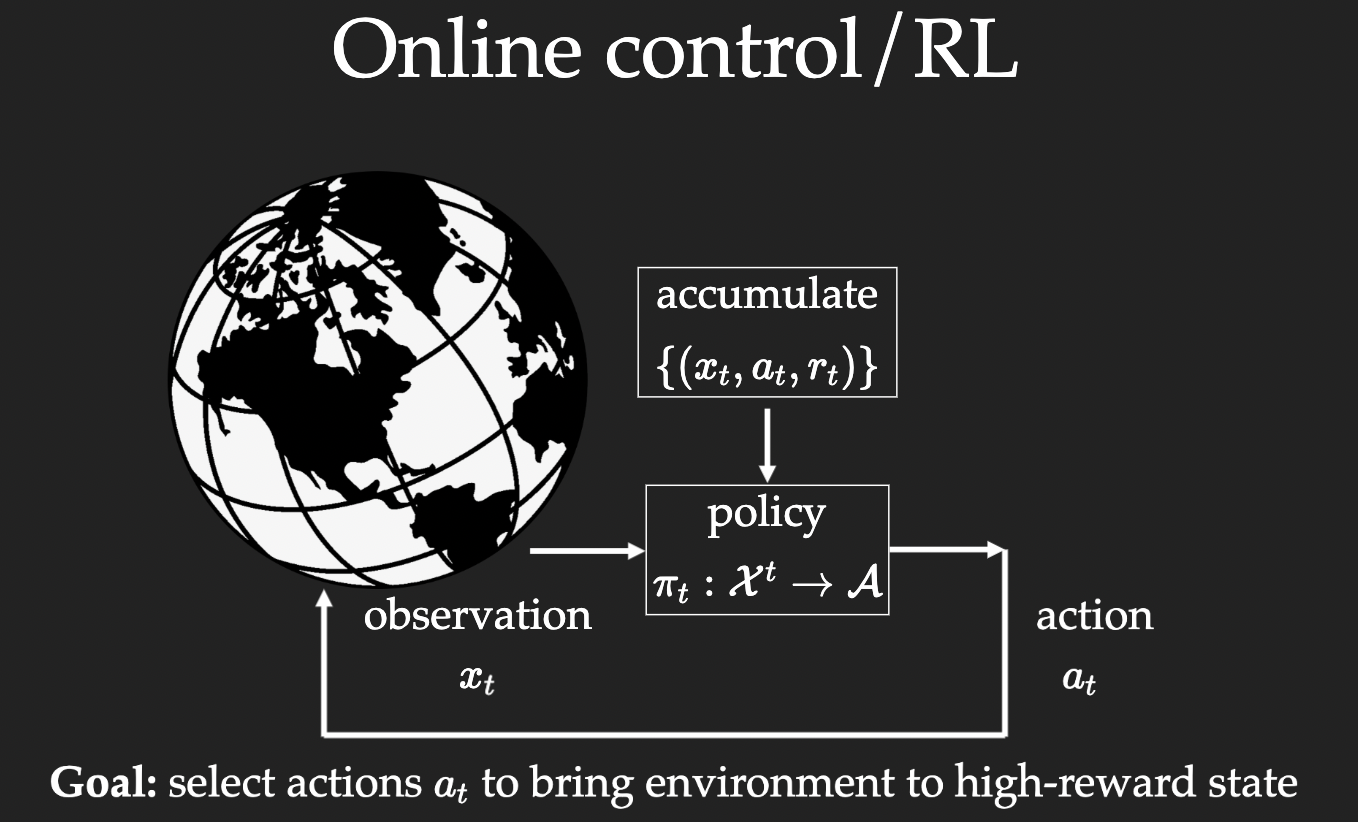
\includegraphics[width=\linewidth]{Online_control.png}
\caption{The Reinforcement Learning framework}
  \label{fig:reinforcement_learning_framework}
\end{marginfigure}

% \begin{figure}[h]
% \centering
% 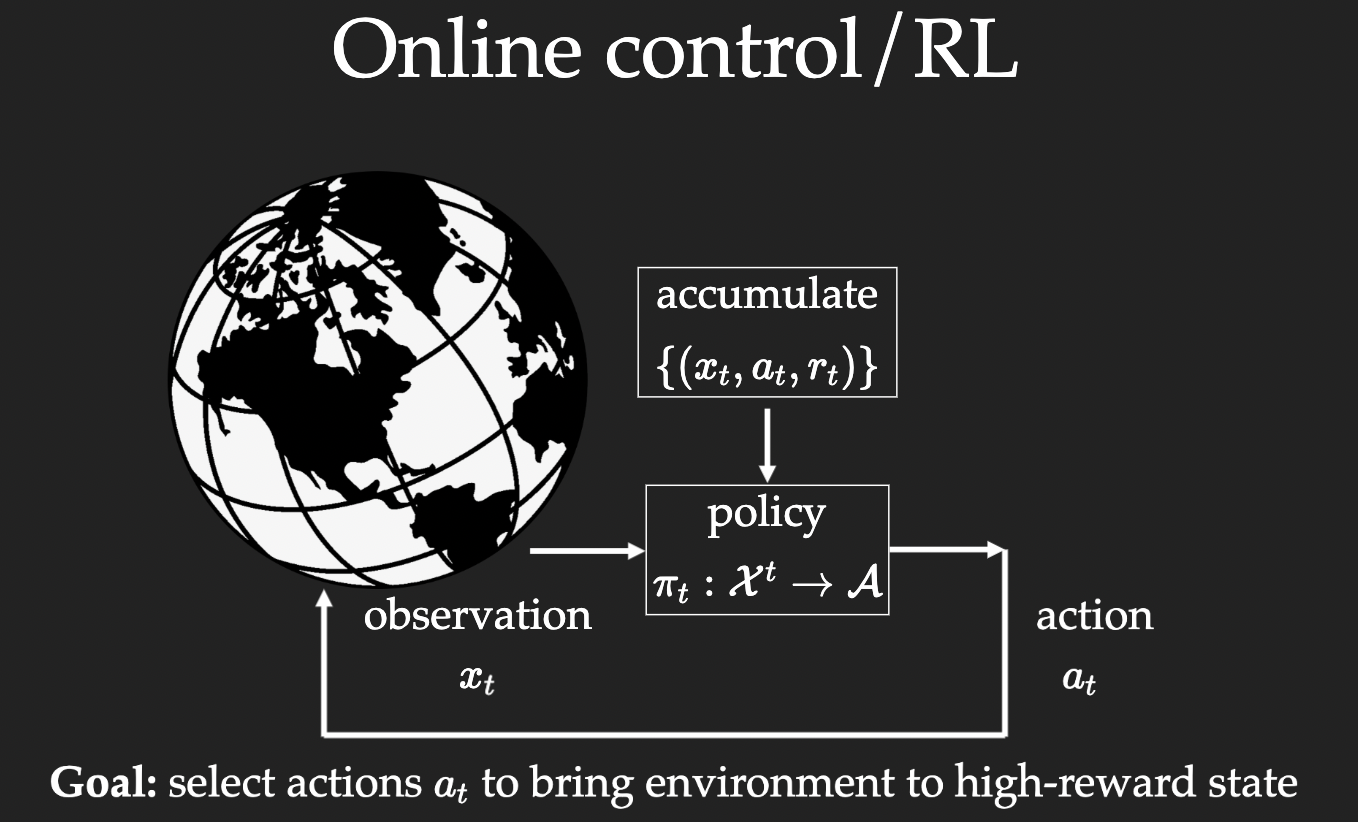
\includegraphics[width=\linewidth]{Online_control.png}
% \caption{The Reinforcement Learning framework}
% \end{figure}\\
Finally, in the setting of Online Control/Reinforcement Learning, we are still in the context of an accumulation of data points that we use to progressively update a policy. However, the big difference with the previous setting is that the environment changes with respect to our actions. We observe a state $x_t$ from a distribution $\chi_t$, pick an action $a_t$ based on our policy $\pi_t$, observe a reward $r_t$ that we use to update our policy. At time $t+1$ however the new state of our environment $x_{t+1}$ is coming from a distribution $\chi_{t+1}$.

\marginnote{Originally scribed by Eliot Shekhtman \& Yann Hicke on August 22nd, 2022}

% \part{Prediction}
\graphicspath{ {./1-supervised-learning/} }

\chapter{Supervised Learning}


As stated earlier, in the supervised learning framework, the goal is to train a model to learn a relationship between datapoints and their corresponding labels from a sample of datapoints drawn i.i.d. from some fixed distribution $\mathcal{D}$. To evaluate the accuracy of our model, we define a loss function which evaluates how dissimilar a model's prediction is on a datapoint from the truth.


In supervised learning, training data is used to train a model, and a trained model can make predictions on observations. The goal is to learn predictions that are close to the true (often unobserved) $y$.

\begin{figure}
\centering
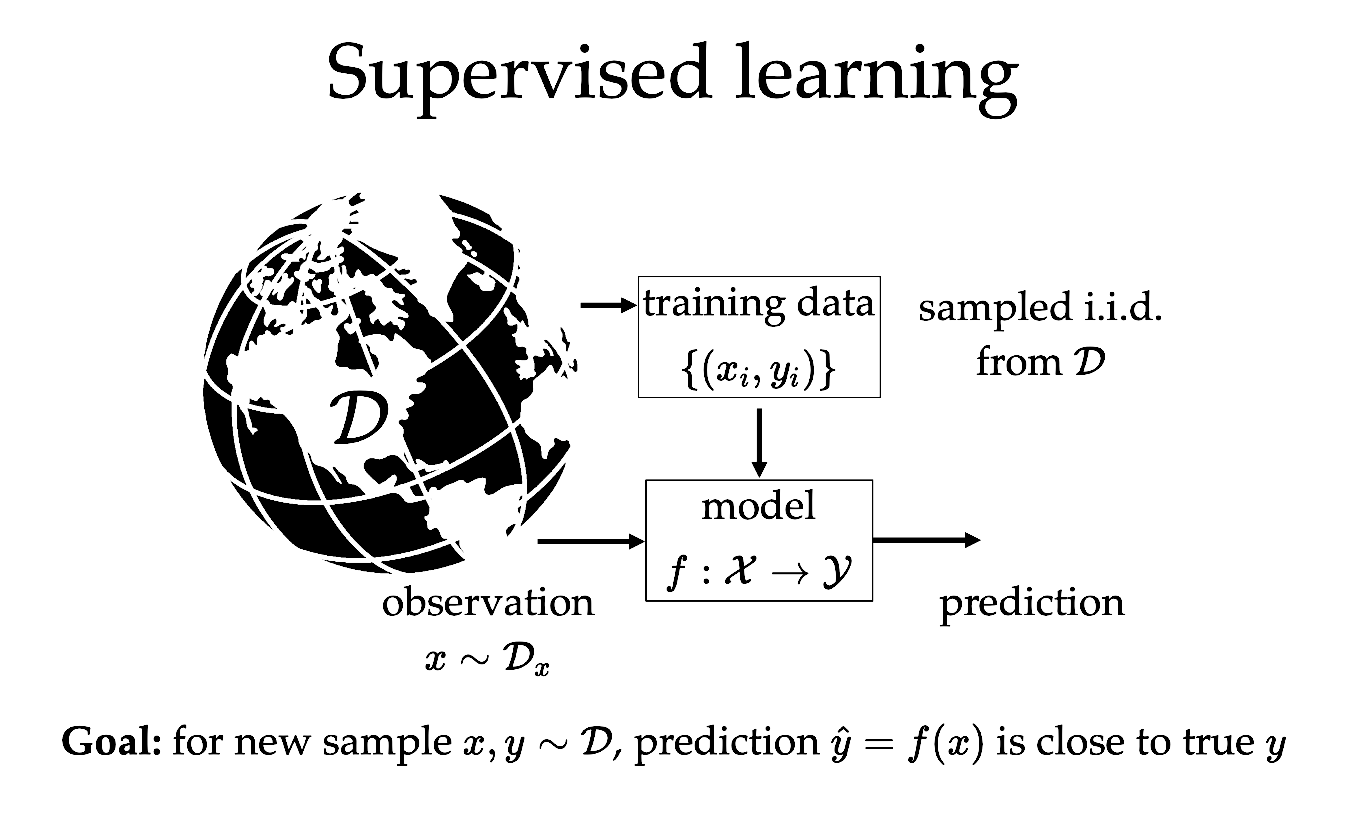
\includegraphics[width=3in]{graphics/sup_learning.png}
\caption{Supervised Learning, from the Lecture 1 slides.}
\end{figure}

The goal of supervised learning can be formalized as a risk minimization problem.
Given some user defined loss function $\ell$, the goal in risk minimization is 

\begin{equation}
\min_{p \in \mathcal{P}} \mathcal{R}(p) = \mathbb{E}_{x, y \sim \mathcal{D}} [\ell(y, p(x))]
\end{equation}

where $\mathcal{D}$ is a dataset and $\mathcal{P}$ is the set of candidate models. When we approximate $\mathbb{E}_{\mathcal{D}}$ with an actual dataset and evaluate $R$ over real data points then this becomes empirical risk minimization.
The process of supervised machine learning can thus be encapsulated in two things: defining a loss, and conducting risk minimization. 

\section{Predictions and Errors}
A loss function $\ell(y, \hat{y})$ measures the loss when a model predicts $\hat{y}$ when the true label is $y$; this function varies on the setting and desired characteristics of the learning algorithm.  

\begin{table}[ht] 
\centering
  \fontfamily{ppl}\selectfont
  \begin{tabular}{p{0.3\linewidth} | p{0.7\linewidth}}
    \toprule
    Classification Loss & Usage \\
    \midrule
    \textbf{Zero-One Loss} $\mathbb{1}[y\not=\hat{y}]$ & Classification accuracy; this loss is non-continuous and impractical to optimize because of its non convexity. \\
    \textbf{Hinge Loss} $max(0, \hat{y} - y)$ & Denotes the margin between the linear separator and its closest points on either class, it is convex but isn't differentiable at $\hat{y}=y$.  This is used in the standard SVM. \\
    \textbf{Log Loss} $log(1 + e^{-\hat{y}y})$ & Outputs are well-calibrated probabilities for each class; this loss function is used for logistic regression. \\
    \textbf{Exponential Loss} $e^{-\hat{y}y}$ & Used in AdaBoost, misprediction loss increases exponentially: this can converge quickly or cause issues when the data is noisy. \\
    \bottomrule
  \end{tabular}
  \caption{Different classification losses can be picked to handle different optimization schema.}
  \label{tab:normaltab}
  %\zsavepos{pos:normaltab}
\end{table}

\begin{table}[ht] % if you can make the equation and name work well on the same line, idk how to do that tho it isn't that important
  \centering
  \fontfamily{ppl}\selectfont
  \begin{tabular}{p{0.3\linewidth} | p{0.7\linewidth}}
    \toprule
    Classification Loss & Usage \\
    \midrule
    \textbf{Mean Absolute Error} $\left|\hat y-y\right|$ & Estimates median label: this loss function is convex and less sensitive to noise but it isn't differentiable at 0. \\
    \textbf{Squared Loss} $\begin{aligned}
&\left(\hat y - y\right)^{2} 
\end{aligned}$ & Estimates mean label: this loss function is convex and differentiable everywhere, but it's sensitive to outliers and noise. \\
    \bottomrule
  \end{tabular}
  \caption{Different regression losses can also be picked to handle different optimization schema.}
  \label{tab:othertab}
  %\zsavepos{pos:normaltab}
\end{table}

% \includegraphics[width=\linewidth]{graphics/Loss_reg.png}

%   - regression: |^y-y| MAE, (^y-y)^2 MSE both convex, square is also smooth 


\marginnote{Risk can be seen as a natural lens to quantify a model's predictive power.} 

The loss may vary from sample to sample. The risk of a predictor $p$ over a distribution $\mathcal{D}$ is the expected (average) loss. Risk is mathematically defined in the following way:

$$\mathcal{R}(p)=\mathbb{E}_{x, y \sim \mathcal{D}}[\ell(y, p(x))].$$

In supervised machine learning, we consider the best model to be the one with the lowest risk.
The following claim describes when
the best prediction for some feature $x$ comes from the conditional expectation of the label $y$ given $x$.
\begin{claim}\label{claim:condition_exp}
    The predictor with the lowest possible risk is: 
    \begin{itemize}
        \item $\mathbb{E}[Y \mid X]$ for squared loss
        \item $1\{\mathbb{E}[Y \mid X] \geq t\}$ for $0-1$ loss, with threshold $t$ depending on $\mathcal{D}$
    \end{itemize}
\end{claim}
If all our data were stored in a large table, we could compute the conditional expectation as follows: First, find all the entries with matching features $x_i=x$, and then average the corresponding labels $y_i$.
In practice, we rarely have access to labelled data of the entire distribution---instead, we only have some samples. 
Furthermore, the feature description $x$ may be so rich and high dimensional that nothing in our finite dataset exactly matches it.
We will consider both of these issues later in this chapter.


Loss determines trade-offs between errors, as some variation might be truly unexplainable or our feature set might not be complete!  An example of this might be attempting to predict whether a person in a picture is sitting or standing simply based on the position of their face in a frame.  This feature set clearly won't give us a 100\% accurate classifier. 

When we classify, we might classify things correctly (predict stand for a standing person, sit for a sitting person), and here it would make sense for the loss to be 0; however, what if we predict standing for a sitting person versus sitting for a standing person?  Would we want to assign both these situations the same loss?  We must make this decision based on the motivation of building our model, and based on our priorities.  

An example of where we might want to bias this is the proposed idea for skipping TV advertisements in the future: the idea proposed that people could stand up during an ad, and a camera would capture this movement and skip it.  Perhaps we care about customer satisfaction, so we might want to give a higher loss to predicting sitting when the person stands, so customers wouldn't return TVs which force them to stand multiple times to skip an ad.  Perhaps we care more about advertiser satisfaction, so we might want to give a higher loss to predicting standing when the person sits, so we can ensure that consumers won't accidentally skip ads which they might have acted upon while idly sitting.  There are many things to consider for each decision while designing a loss function!

In many domains, decisions have moral and legal significance, and harms can occur at many levels.  As machine learning is applied to a variety of settings, we must analyze several possible ways that machine learning algorithms might cause harm in application.  \\

\begin{itemize}
    \item Correctness: who is burdened by errors?
    \item Stereotyping: which correlations are permissible?
    \item Specification: who is left out?
\end{itemize}

An additional component of these issues is that we don't often have access to the entire population $\mathcal D$ and instead use a finite dataset; we revisit this issue towards the end of the chapter.





\section{Fairness Metrics}

Consider the problem of targeted job ads\footnote{\url{https://www.theverge.com/2018/10/10/17958784/ai-recruiting-tool-bias-amazon-report}}, where we want to tell targeted users that we are hiring a programmer. If we use demographic information and browsing history as our input features $x_i$ and whether or not the user clicked (1) or not (-1) as our label $y_i$, we can use the following linear model to determine whether or not to serve ads to future users.

$$\hat{\theta} = \argmin \sum_{i=1}^{N} (-\theta^Tx_i \cdot y_i)_+ \hspace{1cm} \hat{f}(x) = \mathbb{1} \{\hat{\theta}^Tx \ge t\}$$

However, if we optimize this model, we may find that the index of $\hat{\theta}$ corresponding to ``visited website for women's clothing store'' is negative, which implies some sort of bias in the model. We can try to resolve this by removing the feature for women's clothing, but this will just result in other features being selected that may result in biased models. Clearly, removing features that are potentially problematic is not a solution, and this phenomena is known as ``no fairness through unawareness.'' 

\subsection{Statistical Classification Criteria}
\begin{marginfigure}
\centering
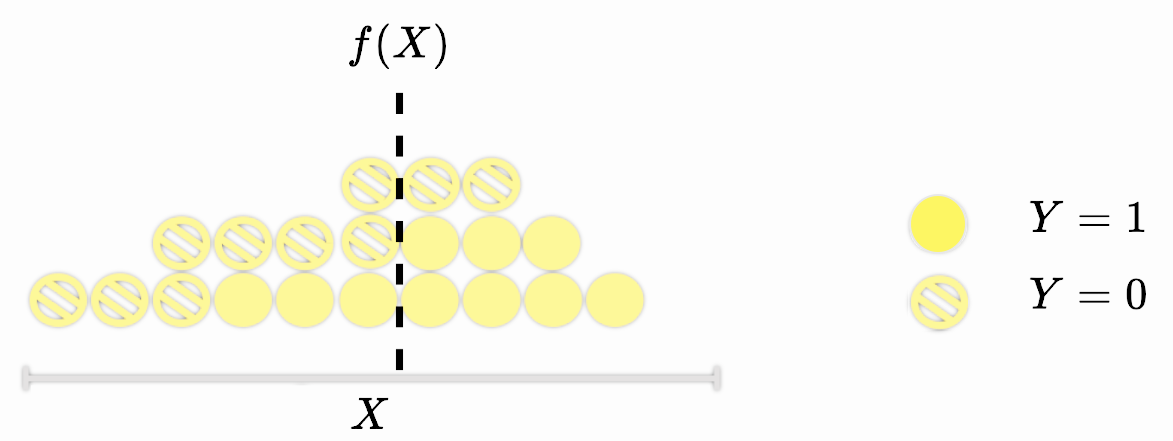
\includegraphics[width=\linewidth]{graphics/example.png}
\caption{Examples of statistical classification criteria.}
\end{marginfigure}
A key component of measuring fairness is understanding what and when the model is predicting. 
Here we demonstrate some metrics that describe this along with an example:
\begin{center}
\begin{tabular}{ ||c | c|| }
 \hline
 Accuracy: $\mathbb{P}(\hat{Y} = Y) = 0.75$  & Positive Rate: $\mathbb{P}(\hat{Y} = 1)= 0.45$ \\ 
 False Positive Rate: $\mathbb{P}(\hat{Y} = 1 | Y = 0)=0.2$ & False Negative Rate: $\mathbb{P}(\hat{Y} = 0 | Y = 1)=0.3$ \\  
 True Positive Rate: $\mathbb{P}(\hat{Y} = 1 | Y = 1)=0.7$ & True Negative Rate: $\mathbb{P}(\hat{Y} = 0 | Y = 0)=0.8$\\
 Positive Predictive Value: $\mathbb{P}(Y = 1 | \hat{Y} = 1)=\frac{7}{9}$ & Negative Predictive Value: $\mathbb{P}(Y = 0 | \hat{Y} = 0)=\frac{8}{11}$\\
 \hline
\end{tabular}
\end{center}

\subsection{Fairness Frameworks}

Here we discuss some frameworks for assessing fairness, a rough idea of the methods to integrate fairness into our model, and the limitations of these methods. Further we mention other instances of discrimination in non classifier models:\\
Due to the biases that risk minimization models develop, we need some additional criteria besides the loss function to achieve fairness. e.g. in the targeted ad example above, the goal is to treat individuals roughly the same across groups. To formalize that, we present 3 criteria that measure this goal:
\begin{itemize}
    \item \textbf{independence:}\\ equalizes positive rate across groups; prediction does not depend on attribute. $\hat{y} \perp a$\\
In the context of the example above, we look at individuals from different racial categories and want to see that predictions look the same, i.e show the ad at equal rate across gender. However, there might be scenarios where this criteria doesn't seem appropriate. As an example, if the predictor is whether somebody is currently pregnant and we would like to show pregnancy-related ad and baby ads. Since there is some underlying difference in pregnancy across genders, this is not the right criteria.
    \item \textbf{separation:}\\ equalizes error rate across groups; given outcome, prediction does not depend on attribute. $\hat{y}\perp a\, \vert y$\\
    in the example, the ad in this case should be displayed to interested users at equal rates across gender. Here by conditioning on the actual outcome, we allow ourselves to account for the fact that certain properties of interest might differ across these protective attributes.\\
    This is relying on what the true qualification level in a population is, or what the underlying distribution of your labels is.
    \item \textbf{sufficiency:}\\ equalizes predictive value across groups; given prediction, outcome does not depend on attribute. $y\perp a\, \vert \hat{y}$\\
    This is saying your predictions are equally useful across all groups by race, or gender or disability, status, or whatever the particular attribute encodes. In the ad example, the users who end up having the ad display to them are interested at equal rates across gender.\\
    This is focused less on the truth of the population, and more on the truth in the model, which is what we're designing. We just want to improve that.
\end{itemize}
\subsection{Achieving non-Discrimination Criteria}
to achieve these fairness criteria we need to process data, the methods are:

\begin{itemize}
    \item \textbf{preprocessing:}\\ The benefit of this is diagnostic to the downstream tasks, and it gets rid of any correlations that could otherwise be used, yet it might end up making accuracy hard to achieve. And it requires knowledge of attributes during data pruning.\\
    in the example illustrated in the picture this corresponds to shifting the data itself.
    \begin{figure}
    \centering
    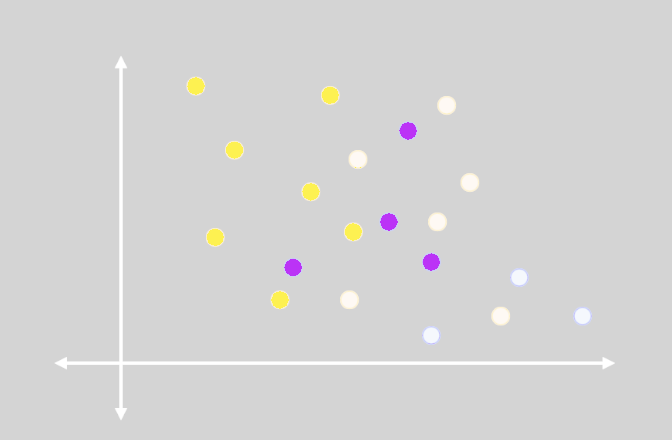
\includegraphics[width=.3\textwidth]{graphics/p1.png}
    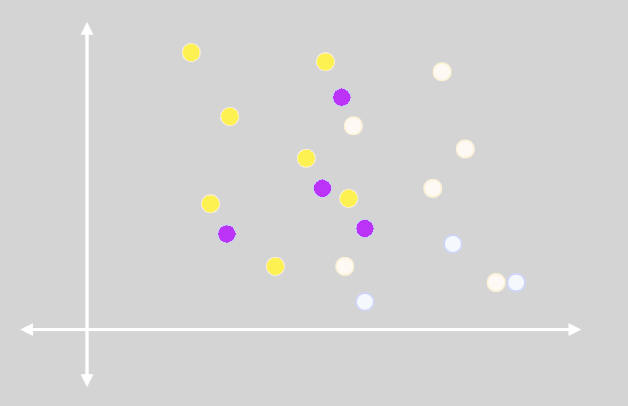
\includegraphics[width=.3\textwidth]{graphics/p2.png}
    \caption{data befor and after pre-processing}
    \end{figure}
    
    \item \textbf{inprocessing:}\\
     Where you change the learning algorithm itself with respect to these criteria, with respect to these criteria, this one will require that you know the protected attribute during training time.\\
     so in the example instead of drawing a linear boundary, we would draw a more complicated looking boundary that will actually satisfy the independence criteria, i.e. equal acceptance rate across groups.
    \begin{figure}
    \centering
    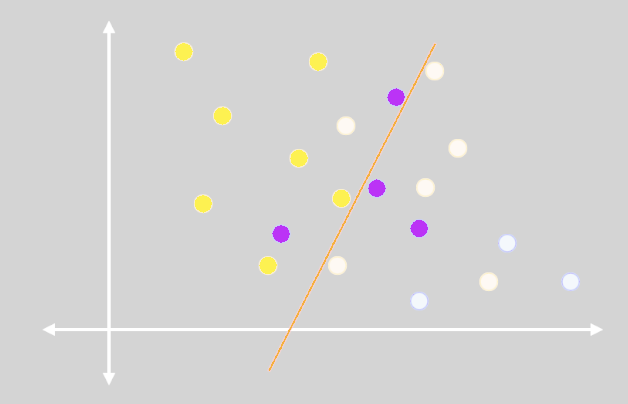
\includegraphics[width=.3\textwidth]{graphics/p4.png}
    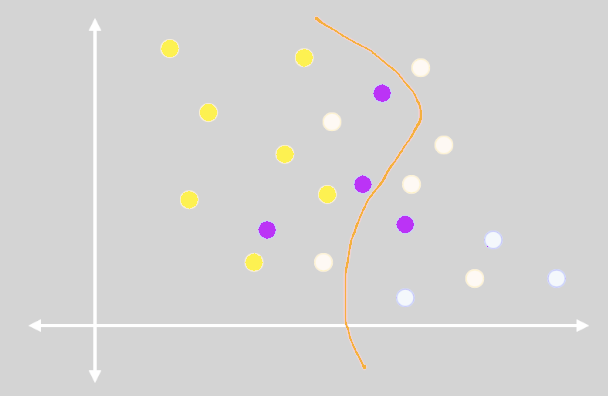
\includegraphics[width=.3\textwidth]{graphics/p3.png}
    \caption{the linear boundary and the boundary after in-processing}
    \end{figure}
    \item \textbf{post processing:}\\ Where we train a model normally and adjust the thresholds(for binary classification) in a group dependent manner after that. This requires incorporating protected attributes at decision time. example.\footnote{See \url{https://research.google.com/bigpicture/attacking-discrimination-in-ml/} for an interactive post processing example.}
    \vspace{10mm}
    \begin{figure}
    \centering
    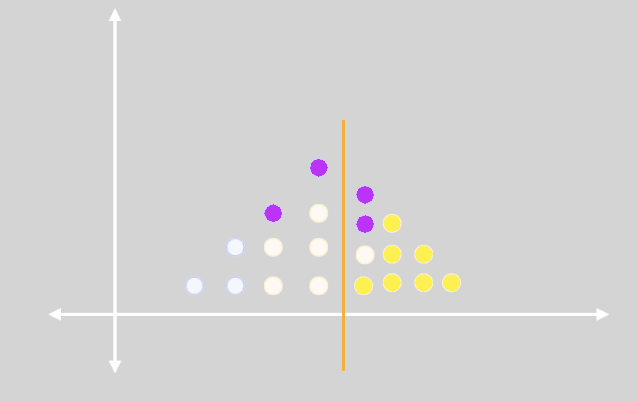
\includegraphics[width=.3\textwidth]{graphics/p5.png}
    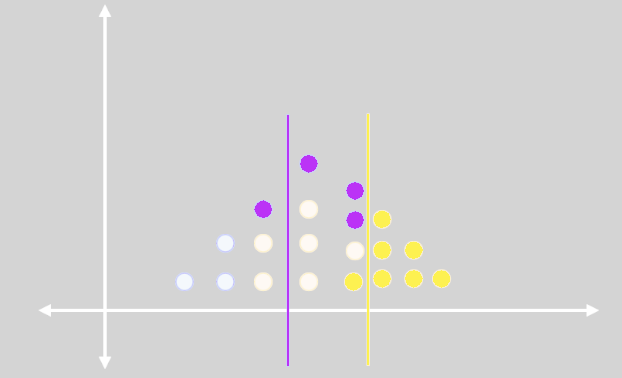
\includegraphics[width=.3\textwidth]{graphics/p6.png}
    \caption{linear classifier without and with post-processing}
    \end{figure}
\end{itemize}
These non-discriminative criteria have some limitations, to mention a few:
\begin{itemize}
    \item Tradeoffs:  It is impossible to simultaneously satisfy separation and sufficiency if populations have different base rates, so we need to decide which ones is of more value to achieve in a specific case.  An example of different base rates would be the example of pregnancy that we discussed. For a controversial example of how sufficiency and separation could be interpreted, refer to the slides.\cite{kleinberg2016inherent}
    \item Observational: Statistical criteria can measure only correlation; whereas intuitive notions of discrimination involve causation, careful modeling is required that distinguishes between the two.\footnote{\url{https://papers.ssrn.com/sol3/papers.cfm?abstract_id=2477899} {big data's disparate impact}}
    \item Unclear legal grounding: While algorithmic decisions may have disparate impact, achieving criteria involves disparate treatment. And you could take either stance in legal battles.
    \item Limited view: focusing on risk prediction might miss the bigger picture of how these tools are used by larger systems to make decisions
\end{itemize}

Fairness related issues happen in non-classifier models as well, there has been such instances in face recognition, image cropping, generative models and search models.

\section{Empirical Risk Minimization: Sample vs Population}\label{sec:sample_vs_population}

Rarely do we have access to the distribution decribing and entire population; instead we must learn from some dataset. The goal of empirical risk minimization is to find 
$$\hat{p} = \min_{p \in \mathcal{P}}\frac{1}{n} \sum_{i = 1}^{n} \ell(y_i, p(x_i))$$

This generally states that we attempt to find the model in a model class which has the least loss over the dataset: the average loss over the training dataset is called the empirical risk and is denoted as $\mathcal{R}_N(p)$. Minimizing our risk over the training dataset is useful since we want a model which reduces the overall risk and our training set is all we have access to. 

\begin{thm}[Fundamental Theorem of Supervised Learning] 
    $$\underbrace{\mathcal{R}(p)}_{risk} \leq \underbrace{\mathcal{R}_{N}(p)}_{empirical\,risk}+\underbrace{\left|\mathcal{R}(p)-\mathcal{R}_{N}(p)\right|}_{generalization\,error}$$

where $\mathcal{R}_{N}$ is the empirical risk of $p$ over some dataset $\mathcal{D}$. In other words, the \textit{true risk} of $p$ is bounded by the \textit{empirical risk} of $p$ plus the \textit{generalization error}.
\end{thm}

the risk associated with our model on the distribution from which its data is sampled from is bounded by the sum of the empirical risk of the model and the model's generalization error. The proof of this theorem merely relies on the fact that the absolute value of a quantity is always at least as big as the value itself. 



\begin{proof}
Reordering terms,

\begin{align*}
\mathcal{R}(p) - \mathcal{R}_{N}(p) &\le |\mathcal{R}(p) - \mathcal{R}_{N}(p)| \\
a &\le |a|\\
\end{align*}

which is true so thus the theorem holds.
\end{proof}

In general, the risk of the learned model depends on the \textit{representation} of models available to the \textit{optimization} algorithm and is bounded by how well the learned model \textit{generalizes}. In the equation for $\hat{p}$, \textit{representation} corresponds to ``$p \in \mathcal{P}$'' since $\mathcal{P}$ is the set of models we are optimizing over and hoping represents the data. \textit{Optimization} corresponds to $\min$ since $\min$ optimizes the objective loss/risk function. Finally, \textit{generalization} corresponds to $|\mathcal{R}(p) - \mathcal{R}_N(p)|$ since this term computes the difference between the true performance of $p$ (including on out-of-sample data points) and the empirical risk over $\mathcal{D}$.

\section{Least Squares Regression (LSR)}

As a case study, let us examine LSR. Linear models might seem limiting at first, but with sufficiently complex kernels\footnote{e.g. the RBF kernel or the neural tangent kernel (NTK). For more, see Ch 4 of Hardt \& Recht, ``Patterns, Predictions, and Actions'' \url{mlstory.org}.} linear models can actually be relatively powerful models. In LSR, the objective is to find $\hat{\theta}$ where

$$\hat{\theta} = \argmin_{\theta\in\mathbb{R}^d} \frac{1}{n} \sum_{i = 1}^{n} (\theta^T x_i - y_i)^2$$

Since the risk (loss) in LSR is the $L_2$ norm and thus is differentiable and strictly convex, finding the optimal solution to LSR is relatively straightforward. 

\begin{definition}[Convexity]
A function $f$ is convex iff $\forall$ pairs of points $a, b$ in the domain of $f$ and $\forall 0 \le t \le 1$,
$f(ta + (1-t)b) \le tf(a) + (1-t)f(b)$.
\end{definition}

\begin{definition}[Strict Convexity]
 A function is strictly convex iff $\forall$ pairs of points $a, b$ in the domain of $f$ and $\forall 0 \le t \le 1$, $f(ta + (1-t)b) < tf(a) + (1-t)f(b)$.
\end{definition}

\begin{definition}[Strong Convexity]
 A function is strongly convex iff $\forall$ pairs of points $a, b$ in the domain of $f$ and for any inner product $\langle\cdot, \cdot \rangle$ and corresponding norm $\| \cdot \|$, $\langle \nabla f(x) - \nabla f(y), x - y \rangle \ge m \| x - y \|^2$. Intuitively, for the Euclidean inner product, this means that the growth of the function is lower bounded by some constant proportional to $m$.
\end{definition}

\begin{figure}
\centering
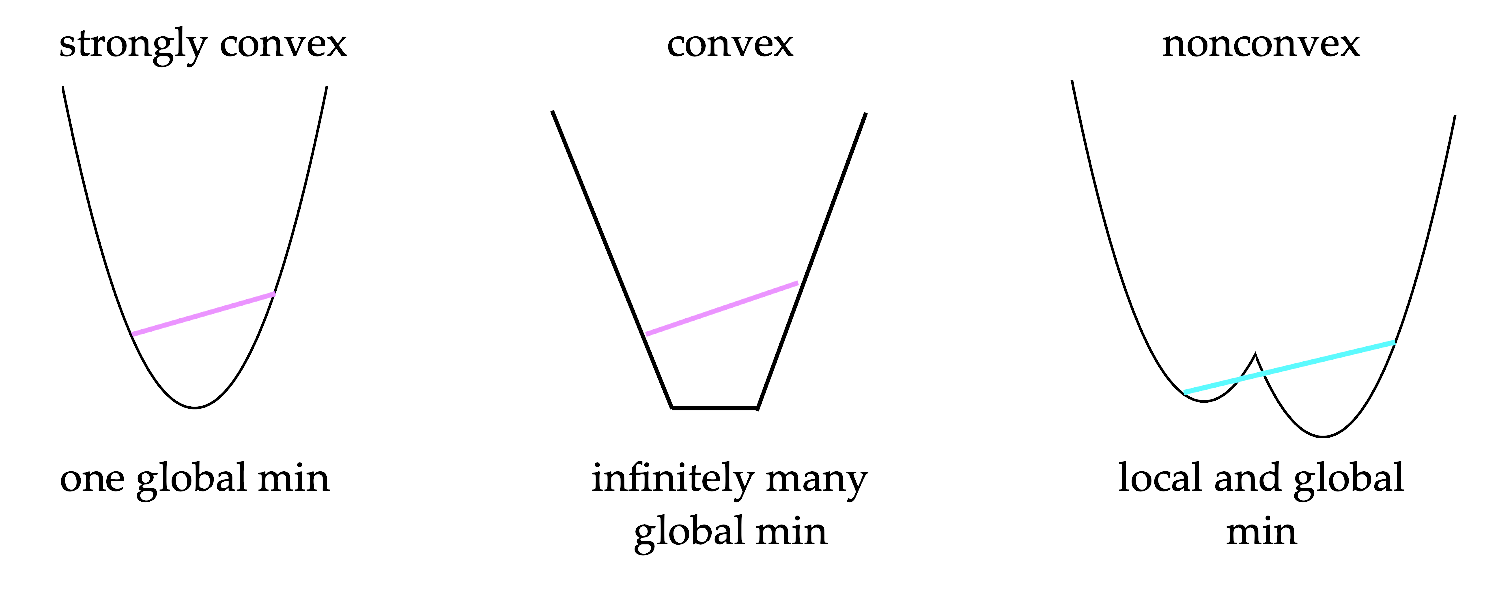
\includegraphics[width=3in]{graphics/convex.png}
\caption{Various functions and their (non) convexity properties.}
\end{figure}

LSR has a closed form solution $\hat{\theta}$ which is pretty rare; most complex models do not have a nice closed form solution. To find the closed form solution of $\hat{\theta}$, consider when the gradient of $\frac{1}{n}\sum_{i=1}^{n}(\theta^T x_i - y_i)$ w/rt to $\theta$ is 0.

\begin{align}
\nabla \frac{1}{n}\sum_{i=1}^{n}(\theta^T x_i - y_i) &= \frac{1}{n}\sum_{i=1}^{n} \nabla (\theta^T x_i - y_i)^2 \\
&= \frac{1}{n} \sum_{i=1}^{n} 2x_i(x_i^T \theta - y_i)
\end{align}

The gradient\footnote{We can move the transposes around since $\theta^Tx_i$ and $y_i$ are scalars.} is equal to 0 when 
$$\sum_{i=1}^{n} x_ix_i^T\hat{\theta} = \sum_{i=1}^n y_ix_i.$$

This is the \textit{first order optimality condition} for LSR. To solve for $\theta = \hat{\theta}$, let $X$ be a matrix where each row is a data point $x_i$ and $Y$ be a matrix where each row is a label $y_i$. Then, the first order optimality condition becomes

$$X^TX\hat{\theta} = X^T Y$$

If $X$ is full rank (i.e. the problem is not underspecified), then $X^TX$ is full rank and thus invertible. 
If $X$ is not full rank (i.e. the problem is underspecified), then we can use the psuedoinverse\footnote{Also called the Moore Penrose Inverse, see \url{https://en.wikipedia.org/wiki/Moore\%E2\%80\%93Penrose_inverse}. The pseudoinverse is denoted with $\dag$.} to get $\hat{\theta}$. Thus, 

$$\hat{\theta} = (X^TX)^{\dag}X^TY = (\sum_{i=1}^{n} x_i x_x^T)^{\dag} \sum_{i=1}^{n} y_ix_i.$$

The pseudoinverse has the nice property of producing the min-norm $\hat{\theta}$\footnote{Since the system is underspecified, there are infinitely many $\hat{\theta}$'s that achieve the minimum risk.}. This can be shown using Lagrange multipliers or projections among other methods. In the case of a fully specified system (i.e. $X^TX$ is invertible) then the pseudoinverse is the inverse and $\hat{\theta}$ is still the min-norm solution since there is only one solution.

Thus, we have derived the empirical risk minimizer for this least squares problem. 
We now consider the population risk. 
To do so, we start with a 
\textit{fixed design} generative model, the features describing the setup are fixed and the labels are determined by:
\begin{align*} 
y_{i} = \theta_{*}^{T}x_{i} + v_{i}
\end{align*}
where $v_{i}$ is i.i.d with a mean of $0$ and variance of $\sigma^{2}$. The population risk is given by
\begin{align*} 
R(\theta) = \frac{1}{n} \sum_{i=1}^{n}\mathop{{}\mathbb{E}}_{yi} [(x_{i})^{T}\theta - y_{i})^{2}]
\end{align*}
Due to the random noise on the labels $y_i$, even the optimal $\theta_\star$ does not have zero risk.
We will consider the excess risk, defined as $R(\theta) - R(\theta_{*})$
In the exercises, you will prove that the fixed design excess risk of the least squares estimate $\hat \theta$ is given by $\frac{\sigma^2 d}{n}$.

This intuitively makes sense as the higher variance the random the noise, the larger the risk. The more dimensions needed will also increase the excess risk displayed as it's more information to gather. Increasing the number of samples will also lower the excess risk to zero as you see a large number of more samples, your understanding of the true distribution will approach the optimal. 





\marginnote{Originally scribed by Eliot Shekhtman \& Yann Hicke on August 22nd, 2022 and Albert Tseng \& Kimia Kazemian on 8/24/2022}

\section{Exercises}
\begin{exercise}
for the same generative model and a new fixed $x_{n+1}$ what is the expected loss $\mathbb{E}_y[(\hat{\theta}^Tx_{n+1}-y_{n+1})^2]$? Can you interpret the quantities?
\end{exercise}
\begin{proof}
\begin{align*}
    \mathbb{E}_y[(\hat{\theta}^Tx_{n+1}-y_{n+1})]
    &=(\hat{\theta}^Tx_{n+1})^2-2\hat{\theta}^Tx_{n+1}\mathbb{E}_y[y_{n+1}]+\mathbb{E}[y_{n+1}^2] \\
    &=(\hat{\theta}^Tx_{n+1})^2-2\hat{\theta}^Tx_{n+1}\theta_{*}^Tx_{n+1}+(\theta_{*}^Tx_{n+1})^2 \\
    &=([\hat{\theta}^T-\theta_{*}^T]x_{n+1})^2\\
    &=([Y^TX(X^TX)^{\dag}-\theta_{*}^T]x_{n+1})^2\\
    &=([(\theta_{*}^TX^T+V^T)X(X^TX)^{\dag}-\theta_{*}^T]x_{n+1})^2\\
    &=(V^TX(X^TX)^{\dag}x_{n+1})^2
\end{align*}
so the expected loss is the squared error in our estimate at $x_{n+1}$, without considering the underlying noise.
\end{proof}

\subsection{Exercise}\label{sec:exercise}
For the same generative model and a new fixed $x_{n+1}$, what is the expected loss $\mathop{{}\mathbb{E}}_{y}[(\hat{\theta}^{T}x_{n+1} - y_{n+1})^{2}]$? Can we interpret these quantities.
\begin{align*} 
\mathop{{}\mathbb{E}}_{y}[(\hat{\theta}^{T}x_{n+1} - y_{n+1})^{2}] \\
= \mathop{{}\mathbb{E}}_{vi}[(\hat{\theta} - \theta_{*})^{T}x_{n+1} + v_{i})^{2}] \\ 
= \mathop{{}\mathbb{E}}_{vi}[(\hat{\theta} - \theta_{*})^{T}x_{n+1}] + (\mathop{{}\mathbb{E}}_{vi}[v_{i}^{2}]) \\ 
= ((\hat{\theta} - \theta_{*})^{2} + var(v_{i}) + (\mathop{{}\mathbb{E}}_{vi}[v_{i}])^{2} \\ 
= ((\hat{\theta} - \theta_{*})^{2} + \sigma^{2}
\end{align*}
These 2 terms can be interpreted as the bias squared (left term) and some irreducible error/noise (right term).
\smallbreak
In the \textit{random design} setting, we take each $x_{i}$ to be drawn i.i.d from $\mathcal{N}$($0$, $\Sigma$) and assume that $v_{i}$ is also Gaussian. The risk is then $R(\theta) = \mathbb{E}_{x,y}[(x^{T}\theta - y)^{2}]$. What is the excess risk of $\hat{\theta}$ in terms of $X^{T}X$ and $\Sigma$? What is the excess risk in terms of $\sigma^{2}, n, d$?
\begin{align*} 
\mathop{{}\mathbb{E}}[R(\hat{\theta}] - R^{*} &= \mathop{{}\mathbb{E}}||(X^{T}X)^{-1}X^{T}v||_{2}^{2} \\
&= \frac{1}{n}\mathop{{}\mathbb{E}}[v^{T}X(X^{T}X)^{-1}X^{T}X(X^{T}X)^{-1}X^{T}v] \\
&= \frac{1}{n}\mathop{{}\mathbb{E}}[v^{T}X(X^{T}X)^{-1}X^{T}v] \\ 
&= \frac{1}{n}\mathop{{}\mathbb{E}}[v^{T}Pv] \text{, where } P = X(X^{T}X)^{-1}X^{T} \\
&= \frac{1}{n}\mathop{{}\mathbb{E}}[tr(Pvv^{T})] \\
&= \frac{\sigma^{2}}{n}tr(P) \\
&= \frac{\sigma^{2}d}{n}
\end{align*}






\end{document}
